\chapter{Website}
\section{Features}
In this project, the only objective of the website was to collect information from the user, and stock them in the database.

When a user went for the first time on the website, he have to sign up, so we can collect informations about the company. After this operation he can access to his control panel where he can:
\begin{itemize}  
\item Create or edit their switchboard
\item Manage operators (the operator are people who will receive the call from the switchboard)
\item Manage the Company's informations
\end{itemize}  



\section{MVC}
The website is based on the Spring technologie,  it follow the MVC rule (Model-View-Controler). the view is separated from the controller and the model.


\section{Overview}
In this project, the website had to be the only way to interact with the server. Through a simplified website, the users have to fill required informations, then they are saved into a database.
\newline

The website is based on \textbf{Spring} technology,  it follows the MVC convention (\textit{Model-View-Controller}). Each layer has its own role in this convention.


\begin{itemize}  
\item The views represents the content the users will be able to see. In our implementation, these files contains special HTML and special tags to allow dynamic contents. 
\item The controllers corresponds to global files 
\item The model represents the database data. It will perform SQL queries to get some data in order to return them as a simplified object to a controller.
\end{itemize}  

Here is a schematic representation of the website architecture

\begin{figure}[!ht]
  \caption{MVC.}
  \centering
    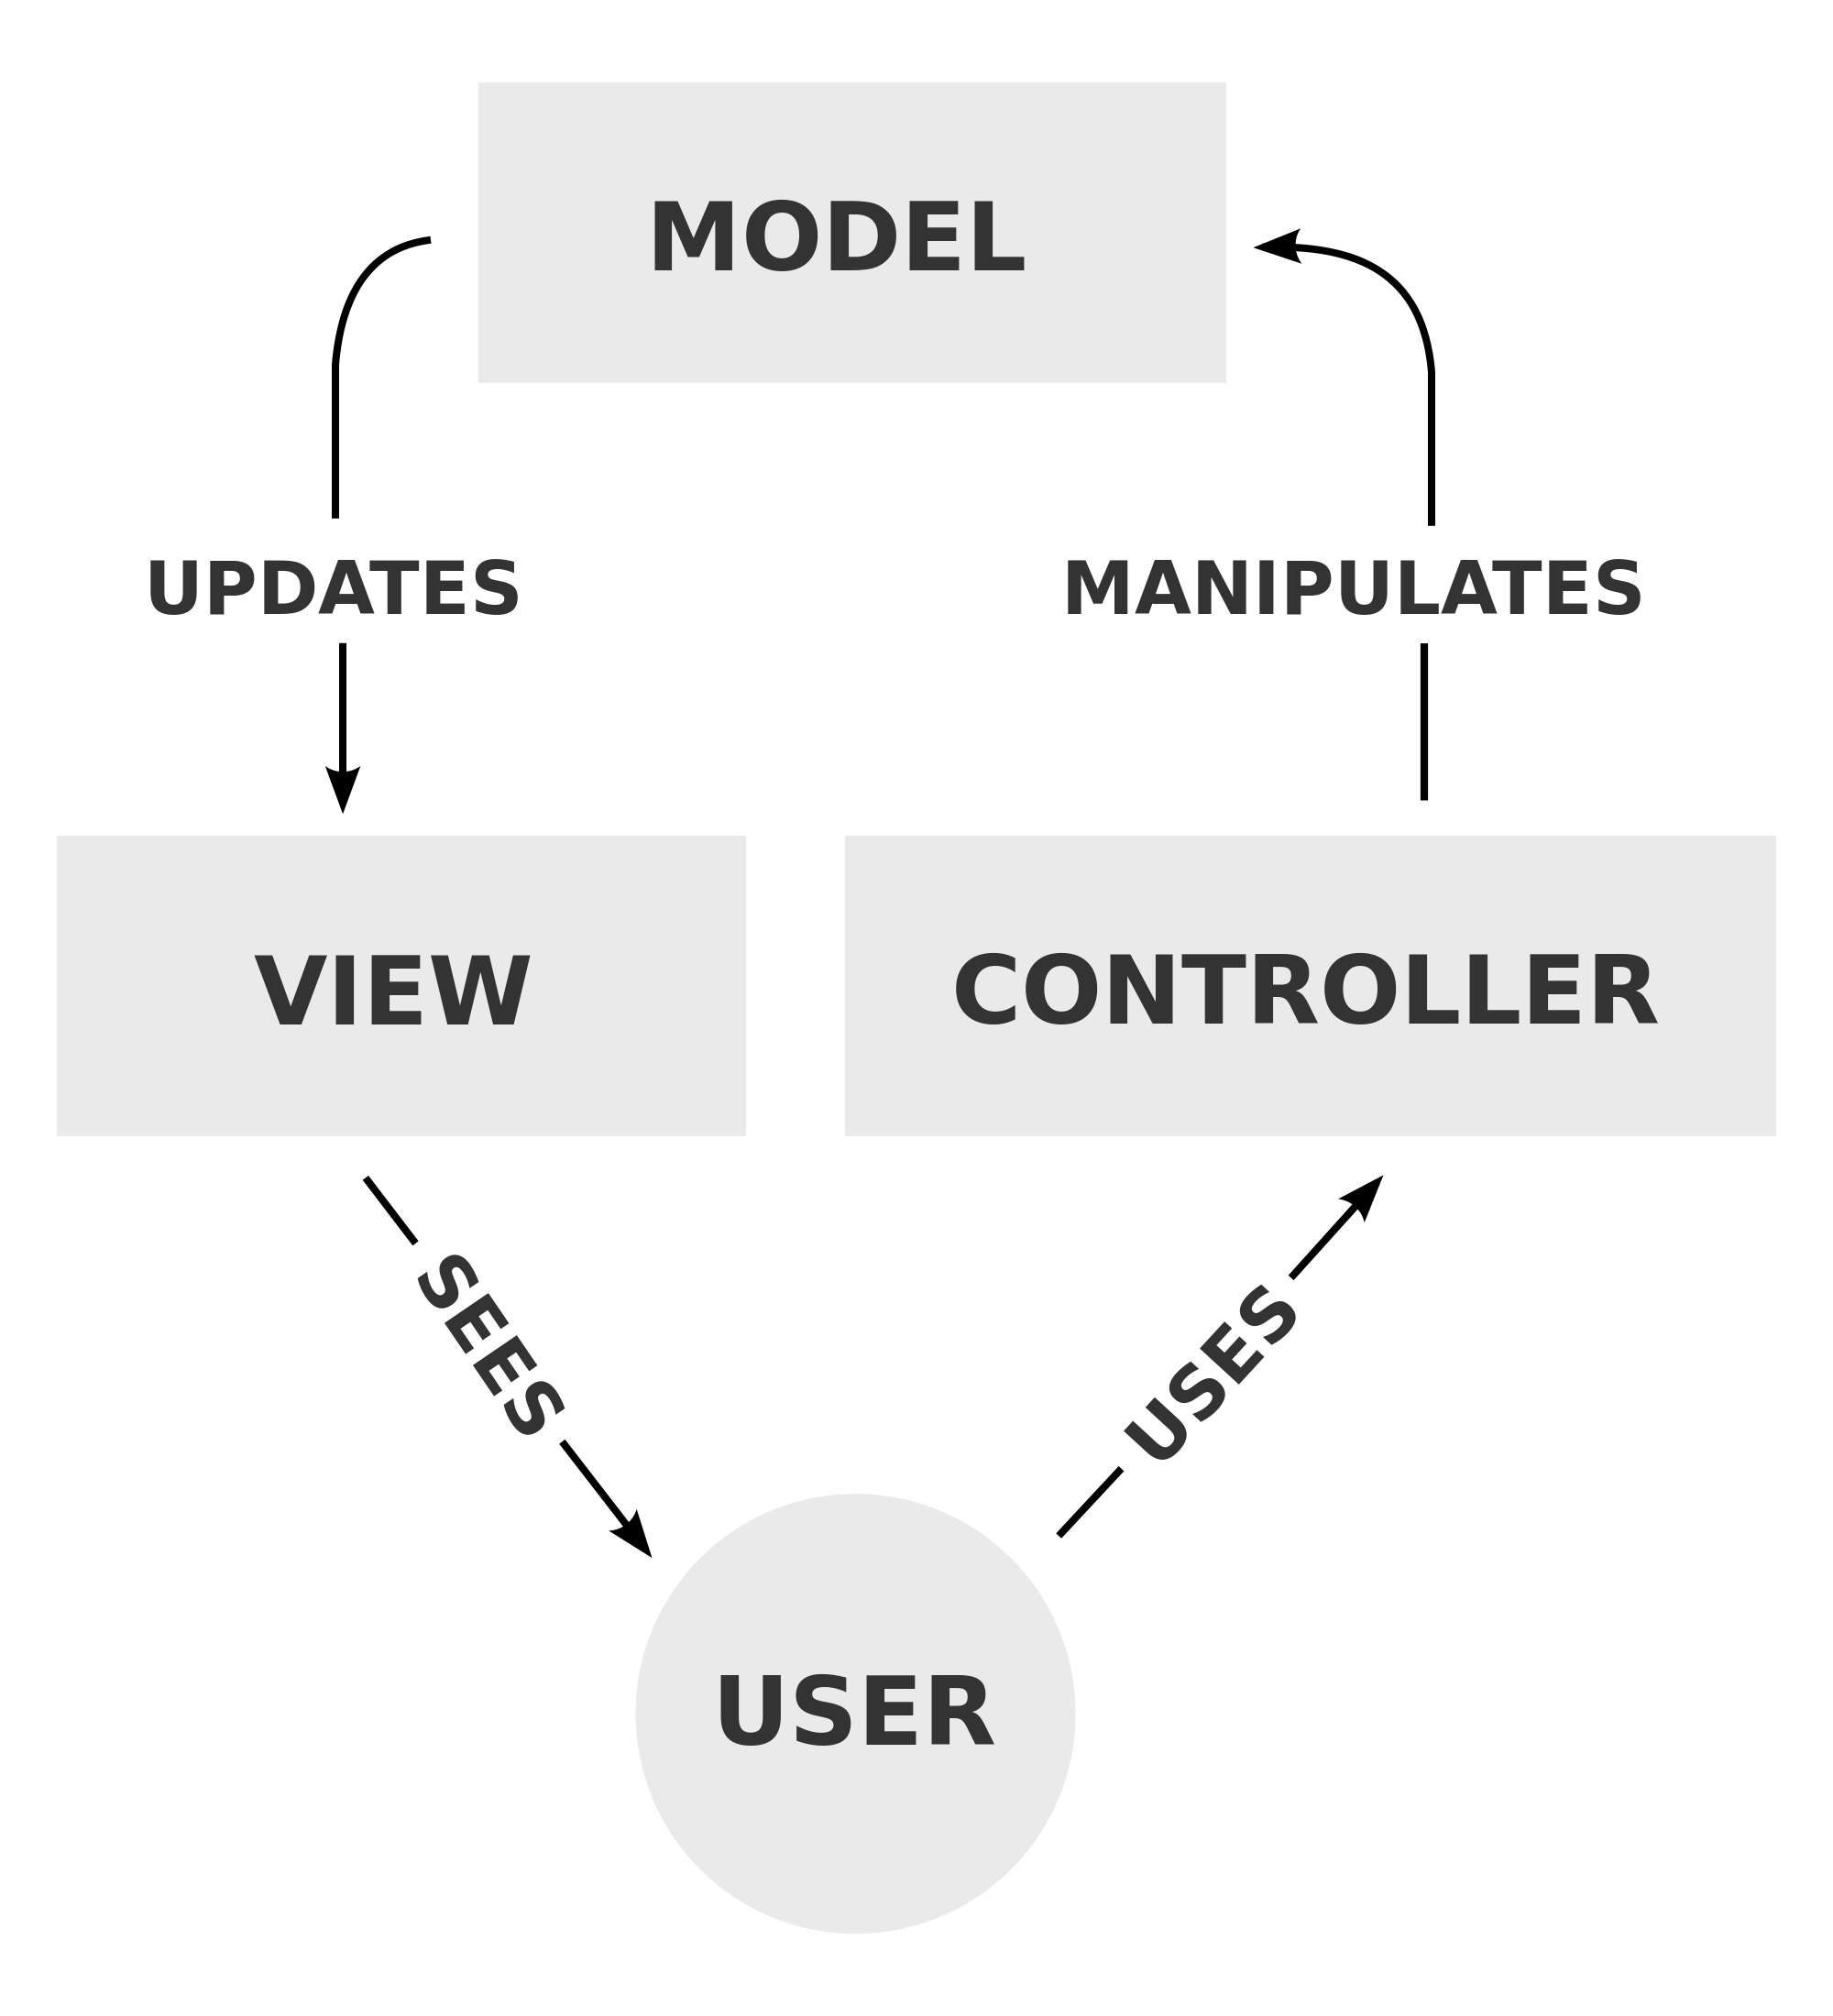
\includegraphics[width=0.5\textwidth]{img/mvc.png}
\end{figure}


\section{Spring application}
\subsection{Why Spring instead traditional J2EE?}

\begin{figure}[H]
  \caption{Logo Spring}
  \centering
    
\includegraphics[width=0.2\textwidth]{img/spring.png}
\end{figure}


Spring is the most popular java framework, It is used in a large parts of professional projects due to his stability, performance and security
It have a lot's of feature such as:

\begin{itemize}  
\item Spring provides easy and secure way to handle Forms, we just give it informations, and he crypt the password and stock it to the datatbase
\item Spring manage the instantiation of the objects without developer worrying about placing instances, when Spring create only one instance and successive calls returns the same object
\item Spring is developed in its core with design pattern as Singleton, Factory, MVC, it's more efficient
\item Spring can manage the dependancy and the configuration of others Frameworks
\end{itemize}  



\subsection{Annotations...}

With Spring and Hibernate, annotations have a very important place in our code, it help the framework to understand the code and apply special action according to theses annotations.
An annotation always begin with '@' and is place above a class, a method or an attribute.

\subsubsection{@Autowired}
@Autowired is a Spring specific annotation, It signal to the framework that it have to inject something special at this location.

\begin{figure}[!ht]
  \caption{@Autowired example}
  \centering
    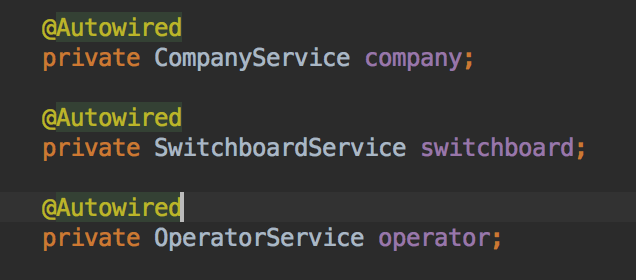
\includegraphics[width=0.9\textwidth]{img/autowired.png}
\end{figure}

In this example, Spring will automatically find the 3 class corresponding to theses declaration, and will automatically inject an object and will stock it in cache. So if we call it after again, we will gain performance because it will not create it again.



\section{Application structure}

\subsection{login}

\begin{figure}[H]
  \caption{Login schematic}
  \centering
    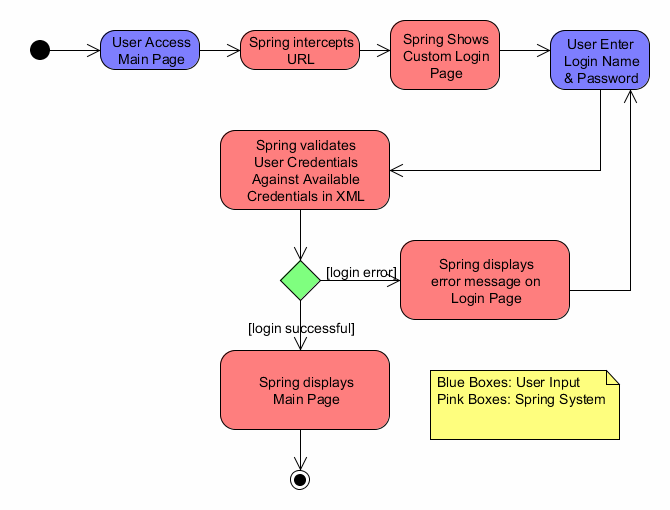
\includegraphics[width=1\textwidth]{img/login.png}
\end{figure}


Here is a schematic representation of a login request processed by Spring





\section{DAO}
\subsection{Controllers}

The controllers are the link between the user and the kernel.
User ask for information : the controller transfer the request to the model, take informations and send them to the view
User give informations : the controller take these informations (after every verifications) and send them to the kernel


\subsection{Hibernate and Models}

The DAO are the link between the program and the database. There are managed by the Hibernate technology, coded in JAVA.
In fact, we have one DAO per entity (switchboard, company...), those files contains functions which returns informations from the database.
\\
\\
Hibernate simplify the interaction with the database, we don't have to use standard SQL interaction.
It works with java object and an hibernate session, we use annotation in the Java class to describe the reproduction of this object in the database,
and we can manipulate this object, transfer it by the session and it will be save on the database.

\section{Services}

We have an other types of files calls "Services", it works with the DAO files.
Their role are to check data send from the application to the DAO, it's avoid errors in the datatbase.
For example it can check data receive from form.


\subsection{View}

The .twig files are an evolution of the HTML files, there are managed by pebble and represents the view of the website.
A .twig file can represent a file, or a part of a file (a layout), like a that we don't have to code every time the same code (like the menu...)
.twig offer something more than a classical html file, it allow to use Java object inside the view, so we can transfer a list and process it directly inside the view.


\subsection{Converters}

\subsection{DTO and Validator}

The DTO are a copy of an entity, which explain constraints, for exemple we can say that an attribute should not be longer than 20 characters...
After we put this DTO inside a view in a form, after validation, the DTO will check every constraints, if everything is correct it will send all the data to the controller in one time,
This method allow a gain of time, network ressources and security.

\subsection{Exceptions}

Exceptions are a special type of class which is call only when something goes wrong...
Java provide a large panel of exceptions, we can use them or create our own Exceptions.
The role of the excerptions are to identified quickly when an error occurred, we have a special name for every exceptions so we can know in a few seconds what is going wrong.


\section{Design}
Due to our inability to make a real design, we chose to download a free open-source design. We found the excellent \textit{AdminLTE2} template suitable for a website like our.
\newline

We cleared and adapted it to our website and needs.
This template is based on the Bootstrap framework which ease the front-end development of a website. Furthermore, the Bootstrap framework is a responsive design: it means our website will be functional on every platform (phone, tablets, computer...) and for all screens size.

\begin{figure}[!ht]
  \caption{AdminLTE2.}
  \centering
    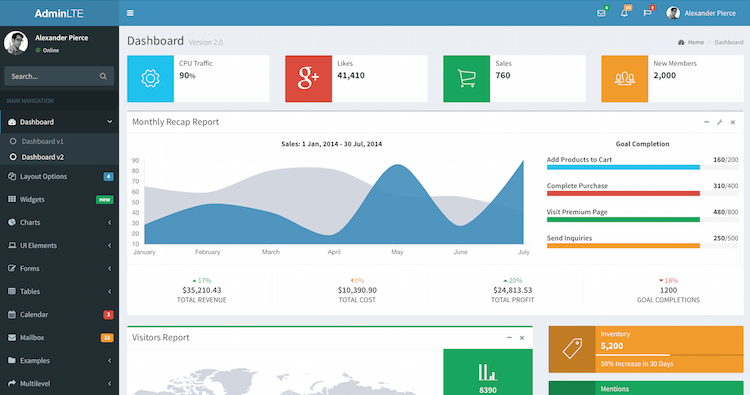
\includegraphics[width=0.9\textwidth]{img/design.png}
\end{figure}





